\documentclass[UTF8,fontset=macnew,xcolor=table]{ctexbeamer}
\usepackage{indentfirst}
\usepackage{color}
\usepackage{xcolor}
\usepackage{enumerate}
\usepackage{listings}
\usepackage{multimedia}
\usepackage{multicol}

\usefonttheme[onlymath]{serif}

\setlength{\parindent}{2em}
\usetheme{CambridgeUS}
\useoutertheme{smoothbars}
\setbeamercolor{normal text}{bg=black!10}
\definecolor{ustcblue}{cmyk}{1,0.8,0,0}

\definecolor{uibred}  {HTML}{db3f3d}
\definecolor{uibblue} {HTML}{4ea0b7}
\definecolor{uibgreen}{HTML}{789a5b}
\definecolor{uibgray} {HTML}{d0cac2}
\definecolor{uiblink} {HTML}{00769E}
\setbeamertemplate{enumerate items}[default]
\setbeamercolor{block body} {bg = uibgray}
\setbeamercolor{block title}{fg = white,bg = uibred}

\renewcommand\lstlistingname{代码}

% \lstset{
%     basicstyle          =   \sffamily,          % 基本代码风格
%     keywordstyle        =   \bfseries,          % 关键字风格
%     commentstyle        =   \rmfamily\itshape,  % 注释的风格,斜体
%     stringstyle         =   \ttfamily,  % 字符串风格
%     flexiblecolumns,                % 别问为什么,加上这个
%     numbers             =   none,   % 行号的位置在左边
%     showspaces          =   false,  % 是否显示空格,显示了有点乱,所以不现实了
%     numberstyle         =   \zihao{-5}\ttfamily,    % 行号的样式,小五号,tt等宽字体
%     showstringspaces    =   false,
%     captionpos          =   t,      % 这段代码的名字所呈现的位置,t指的是top上面
%     frame               =   lrtb,   % 显示边框
%     captionpos          =   b       % caption的位置(填t在上,填b在底部)
% }

\definecolor{mygreen}{rgb}{0,0.6,0}
\definecolor{mygray}{rgb}{0.5,0.5,0.5}
\definecolor{mymauve}{rgb}{0.58,0,0.82}

\lstdefinestyle{Text}{
    language        =   Python, % 语言选Python
    basicstyle      =   \zihao{-5}\ttfamily,
    numberstyle     =   \zihao{-5}\ttfamily,
    keywordstyle    =   \color{black},
    keywordstyle    =   [2] \color{black},
    stringstyle     =   \color{black},
    commentstyle    =   \color{black}\ttfamily,
    breaklines      =   true,   % 自动换行,建议不要写太长的行
    columns         =   fixed,  % 如果不加这一句,字间距就不固定,很丑,必须加
    basewidth       =   0.5em,
}

\lstset{ %
backgroundcolor=\color{white},      % choose the background color
basicstyle=\footnotesize\ttfamily,  % size of fonts used for the code
columns=fullflexible,
tabsize=4,
breaklines=true,               % automatic line breaking only at whitespace
captionpos=t,                  % sets the caption-position to bottom
commentstyle=\color{mygreen},  % comment style
escapeinside={\%*}{*)},        % if you want to add LaTeX within your code
keywordstyle=\color{blue},     % keyword style
stringstyle=\color{mymauve}\ttfamily,  % string literal style
frame=lrtb,
rulesepcolor=\color{red!20!green!20!blue!20},
% identifierstyle=\color{red},
}


\begin{document}
\title[中期报告]{\huge 中期报告}
%\subtitle[副题简称]{论文副题}
\author[中国科学技术大学]{陈思睿 \and 梁恒宇 \and 吕泓涛 \and 汤力宇}
\institute[USTC]{中国科学技术大学}
\date[\today]{\today}
\logo{\textcolor{ustcblue}{\includegraphics[scale=0.25]{ustc_logo_side.pdf}}}
\begin{frame}
    \titlepage
\end{frame}

\section{项目概括}
\begin{frame}{sBPF——基于eBPF结构的安全沙盒}

    \begin{itemize}
        \item 沙盒:一种用于隔离进程的安全机制,用于防御恶意进程和规避系统崩溃。

        \item eBPF: 扩展·伯克利包过滤器(extended Berkeley Packet Filter)
        一种可以安全的在内核态执行用户代码的框架。
        
    \end{itemize}
    
\end{frame}

\section{背景知识}

\begin{frame}{eBPF程序的开发和加载}

    \begin{itemize}
        \item 程序的编写:C或RUST直接编写

        \item 程序的编译:编译器编译成字节码 bytecode
        
        \item 程序的加载:用户态程序向OS请求加载,
        verifier确认安全性,JIT实时编译成本地机械码,放置特定只读内存段
    \end{itemize}
    
\end{frame}

\begin{frame}{eBPF程序的运行}

    \begin{itemize}
        \item 通过钩子触发程序的执行

        \item 系统调用通过helper函数接口实现
        
        \item 局部存储使用mmap和对应helper实现。
    \end{itemize}
    
\end{frame}

\begin{frame}{优点和缺陷}

    \begin{itemize}
        \item 优点:灵活性、安全性、高效率、高兼容性、热升级特性……
        
        试想一下你要魔改你的内核……
    
        \item 缺点:程序的结构、规模和功能类型受限
        
        程序类型、helper函数……
    \end{itemize}
    
\end{frame}

\begin{frame}{eBPF的前景与现状}
    \begin{itemize}
        \item eBPF有着与JVM类似的结构,有正在成为流行的通用框架

        \item 现有的应用:
        \begin{itemize}
            \item bpftrace	动态监测工具,获取目标进程的所有行为
            \item tcpdump	网络包监测工具,提取符合一定条件的所有网络包
            \item InKeV	可编程的网络设备负载均衡和路径选择
        \end{itemize}
    \end{itemize}
\end{frame}

\begin{frame}{沙盒}
    \begin{itemize}
        \item 基本思路是隔离

        \item 面对可疑进程的潜在威胁并保护自己的系统和数据
    \end{itemize}
\end{frame}

\begin{frame}
    \begin{columns}
        \begin{column}{0.3\textwidth}
            {\footnotesize \begin{block}{恶意进程}
                \begin{enumerate}
                    \item Social Engineering
                    \item 栈溢出攻击
                    \item Leak Attack
                    \item 攻击动态加载器
                    \item 利用进程列表攻击其他进程
                    \item 检测沙盒环境并“装死”
                    \item 窃取隐私文件
                    \item 强行植入VNC远程桌面
                    \item 僵尸网络
                \end{enumerate}
            \end{block}}
        \end{column}
    
        \begin{column}{0.3\textwidth}
            {\footnotesize \begin{block}{沙盒}
                \begin{enumerate}
                    \item 局部系统服务
                    \item 检查内存访问
                    \item 局部文件系统
                    \item 设备权限隔离
                    \item 进程隔离
                    \item 限制资源使用量
                    \item 难以感知的监控
                \end{enumerate}
            \end{block}}
        \end{column}

        \begin{column}{0.3\textwidth}
            {\footnotesize \begin{block}{eBPF在沙盒应用的意义}
                \begin{enumerate}
                    \item BPF程序能简单的给内核增加新的安全特性并且易于升级
                    \item 只读代码段不可篡改性不会增加安全漏洞
                    \item 使用BPF可以高效获取资源使用量(现有解决方案)
                    \item 利用钩子直接劫持系统调用,高效且难以被察觉
                \end{enumerate}
            \end{block}}
        \end{column}
    \end{columns}
\end{frame}

\section{一个案例}

\begin{frame}{gVisor的设计思路}
    \begin{columns}
        \begin{column}{0.5\textwidth}
            \begin{itemize}
                \item Ptrace/KVM两种模式
                \item 局部文件系统
                \item Gofer间接访问本机文件系统
                \item Seccomp防止sentry被劫持
            \end{itemize}
        \end{column}

        \begin{column}{0.5\textwidth}
            \begin{figure}[H]
                \centering
                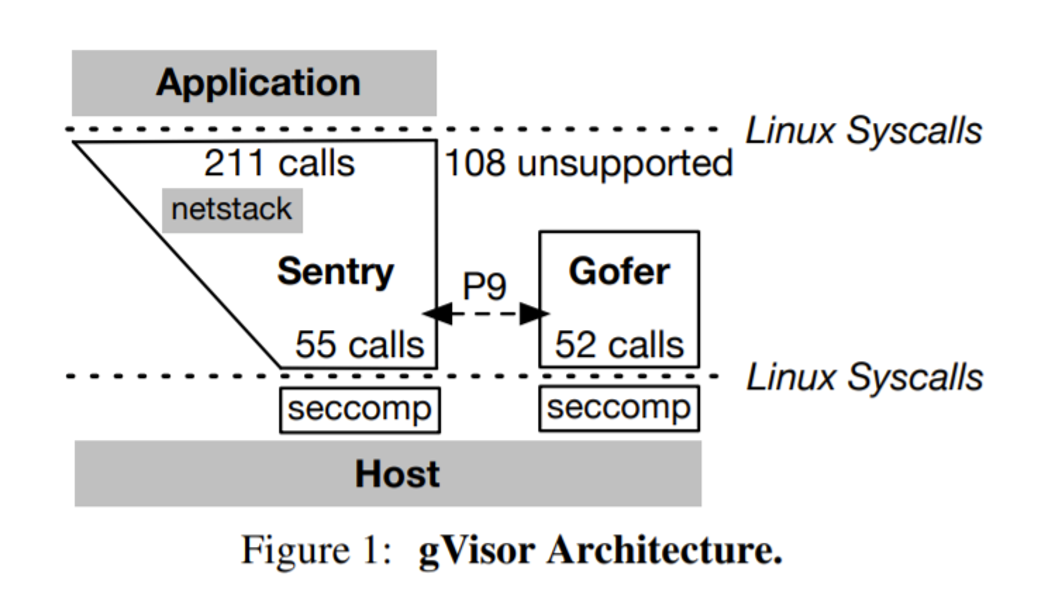
\includegraphics[width=\columnwidth]{pic1.png}
            \end{figure}
        \end{column}
    \end{columns}
\end{frame}

\begin{frame}{gVisor的问题}
    \begin{columns}
        \begin{column}{0.5\textwidth}
            \begin{itemize}
                \item Ptrace效率问题?
                \item Sentry被污染?
                \item 虚拟环境被发现?
            \end{itemize}
        \end{column}

        \begin{column}{0.5\textwidth}
            \begin{figure}[H]
                \centering
                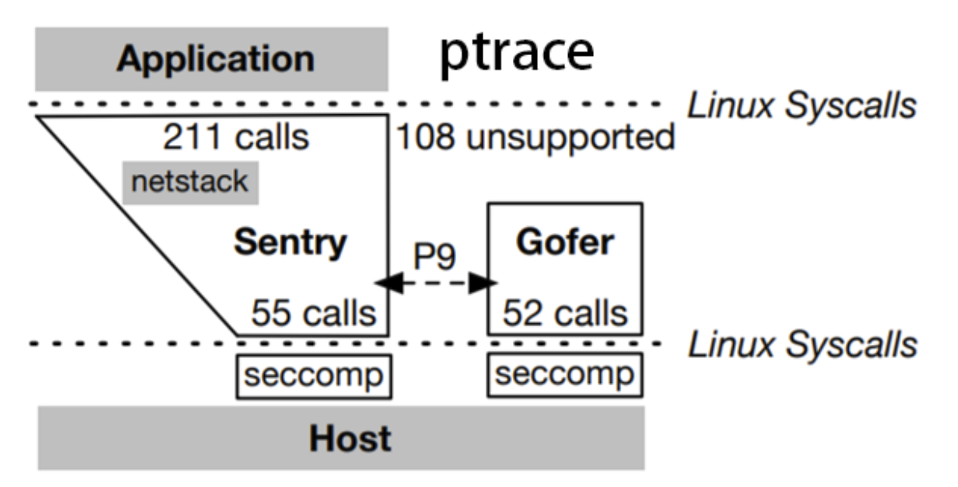
\includegraphics[width=0.8\columnwidth]{pic2.png}
                
\includegraphics[width=0.8\columnwidth]{pic3.png}
            \end{figure}
        \end{column}
    \end{columns}
\end{frame}

\section{项目设计}

\begin{frame}{我们的解决方案——sBPF}
    \begin{figure}[H]
        \centering
        
\includegraphics[width=0.68\columnwidth]{pic4.png}
    \end{figure}
\end{frame}

\section{完成的实践}

\begin{frame}{我们完成的实践——eBPF监控新进程创建}
    \begin{figure}[H]
        \centering
        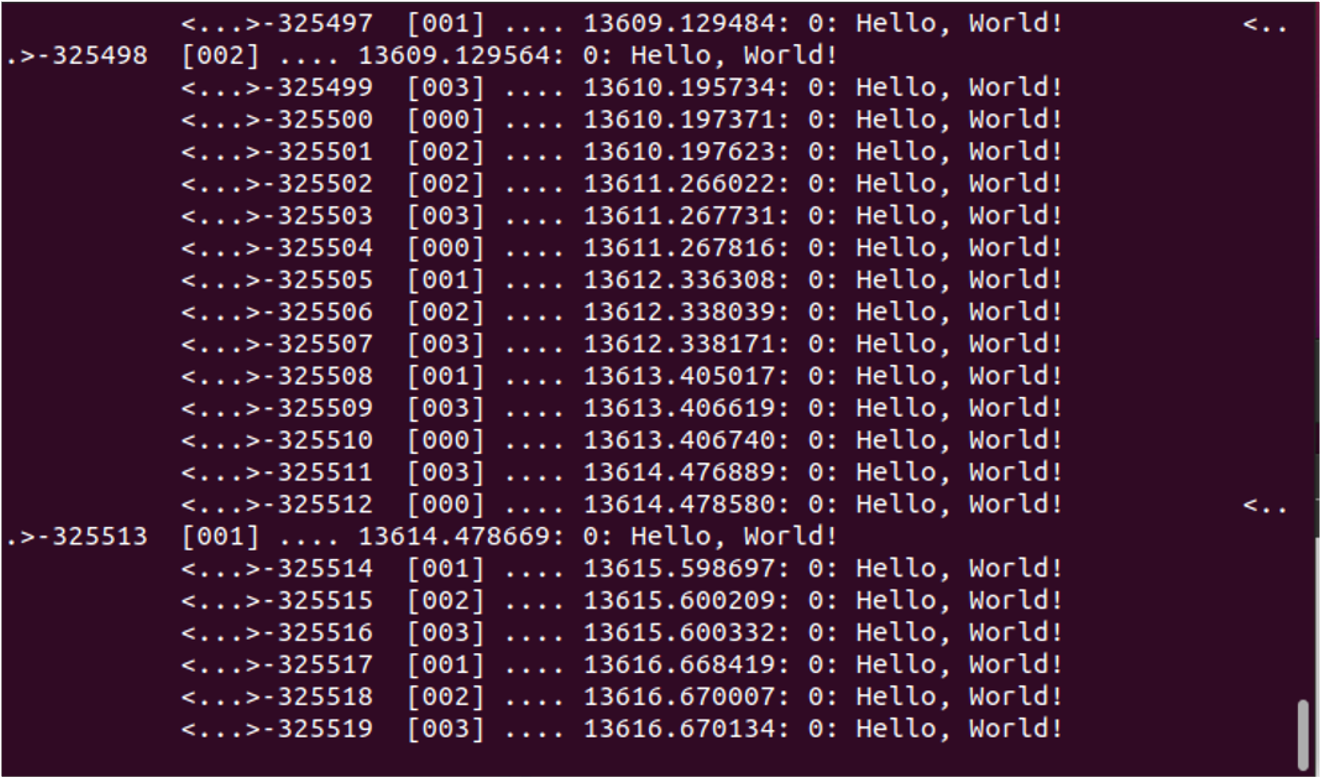
\includegraphics[width=0.68\columnwidth]{pic5.png}
    \end{figure}
\end{frame}

\begin{frame}{eBPF实现的符号跟踪}
    \begin{figure}[H]
        \centering
        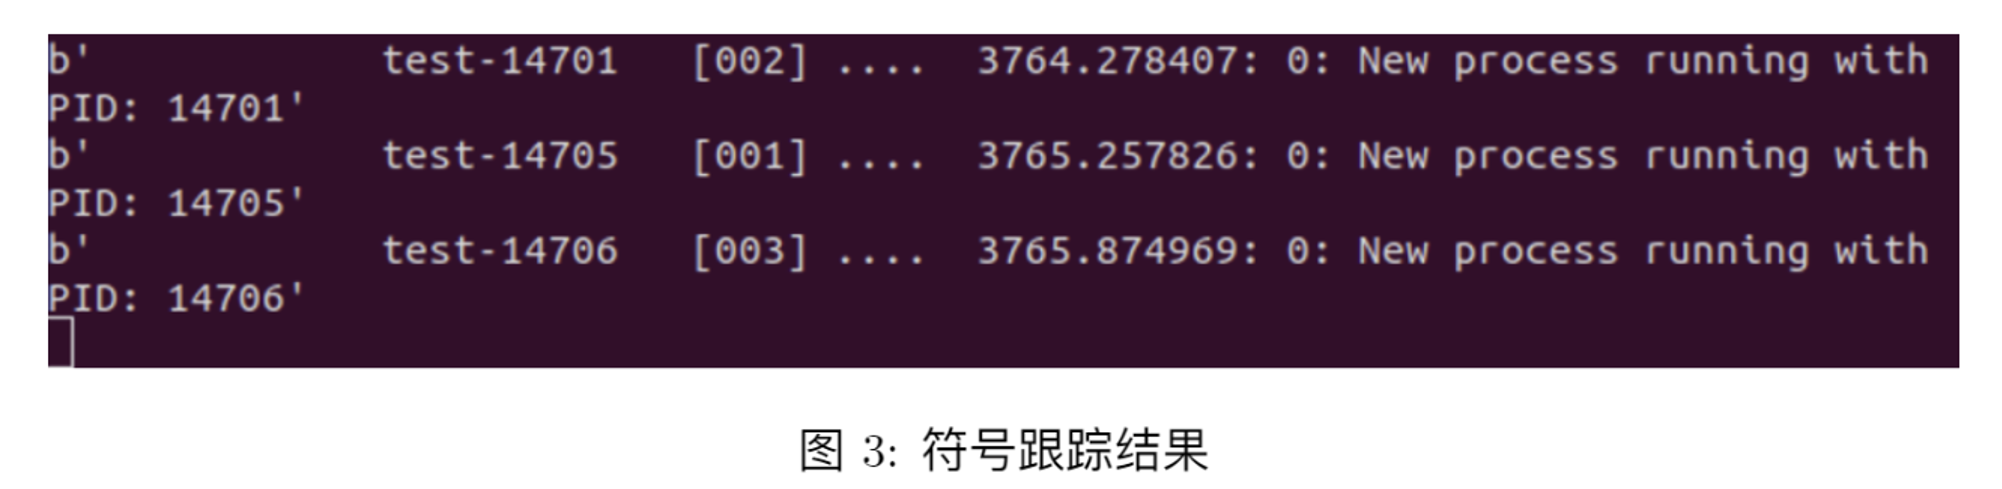
\includegraphics[width=0.72\columnwidth]{pic6.png}
        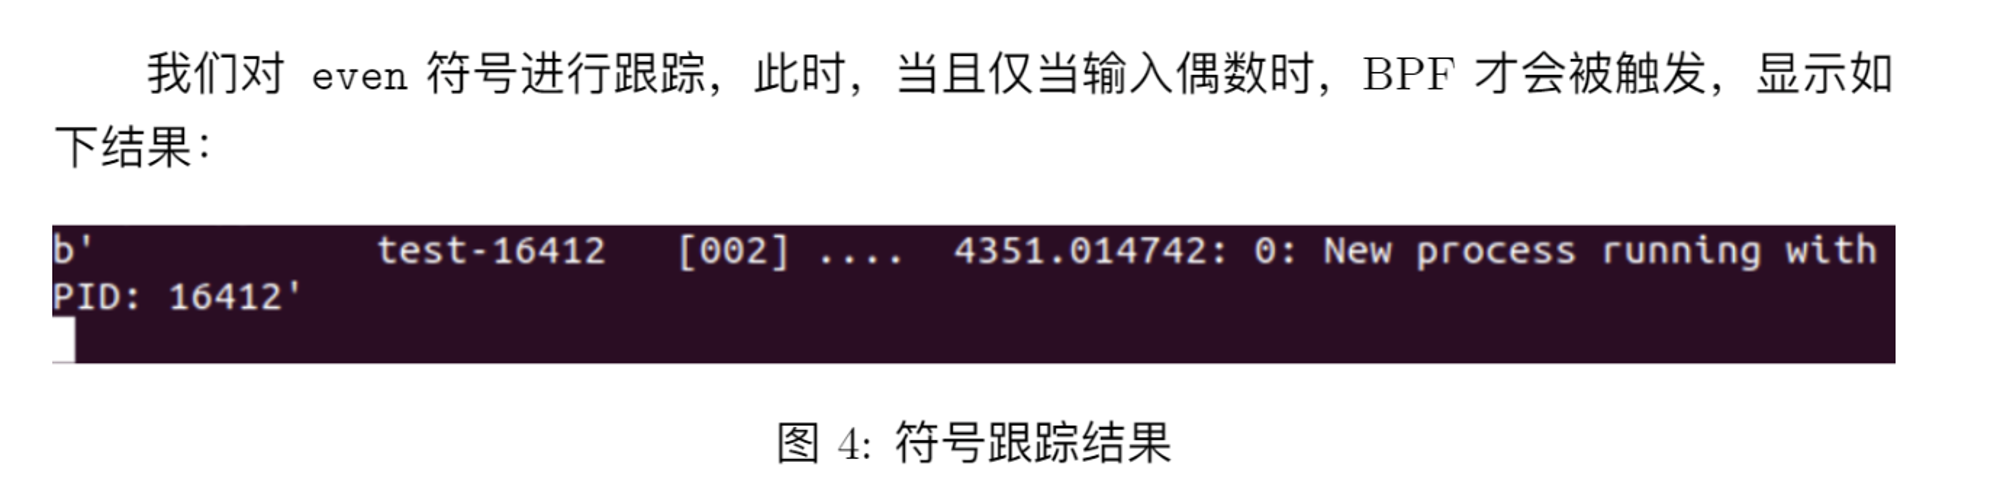
\includegraphics[width=0.72\columnwidth]{pic7.png}
    \end{figure}
\end{frame}

\begin{frame}{seccomp/BPF系统调用过滤与拦截}
    \begin{figure}[H]
        \centering
        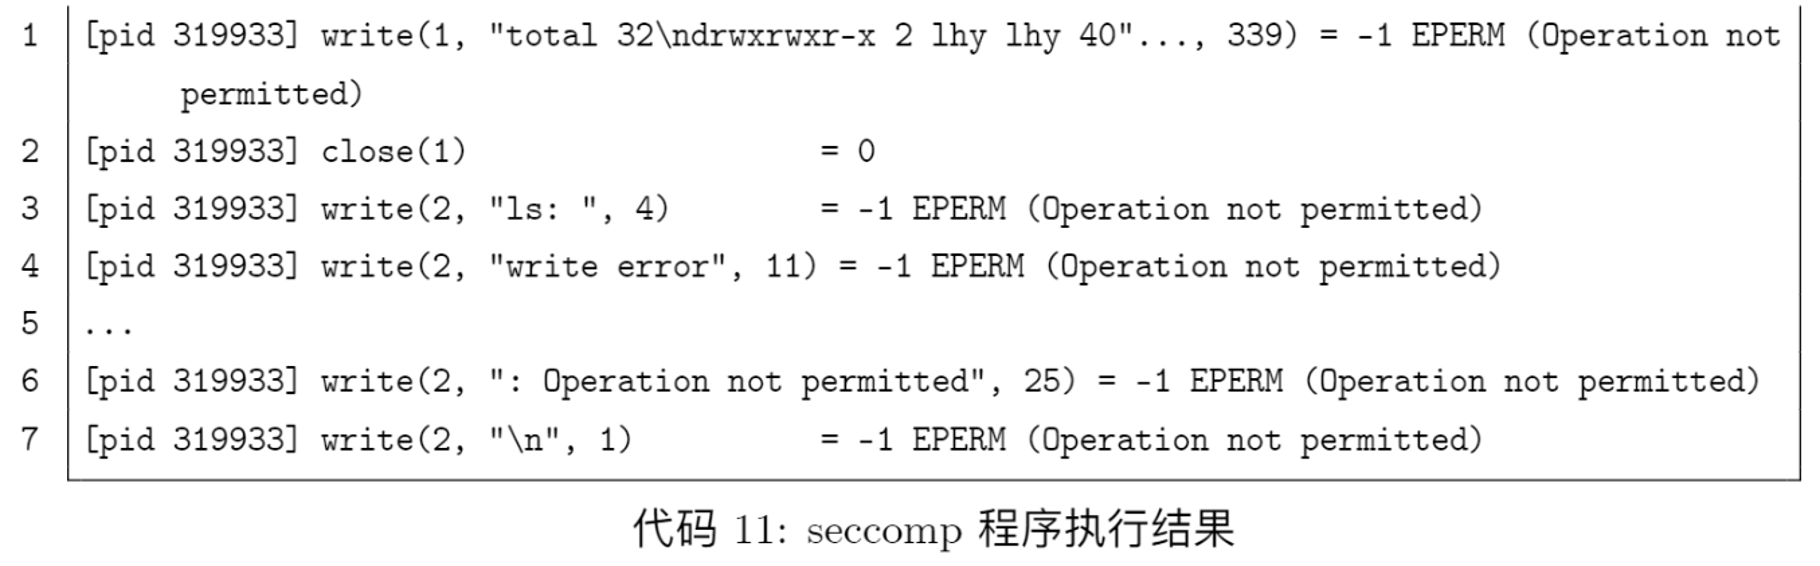
\includegraphics[width=0.8\columnwidth]{pic8.png}
    \end{figure}
\end{frame}

\section{项目规划}

\begin{frame}{规划路线图}
    % Please add the following required packages to your document preamble:
% \usepackage[table,xcdraw]{xcolor}
% If you use beamer only pass "xcolor=table" option, i.e. \documentclass[xcolor=table]{beamer}
\begin{table}[H]
    \begin{tabular}{|c|c|c|}
    \hline 
     & \textbf{一组}     &  \textbf{二组} \\\hline
    阶段一 & eBPF相关接口设计 & 沙盒模块化结构设计 \\\hline
    阶段二 & eBPF相关接口实现 & 沙盒接口设计   \\\hline
    阶段三 & \multicolumn{2}{c|}{沙盒各模块实现}  \\\hline
    阶段四 & \multicolumn{2}{c|}{测试与完善}  \\\hline
    \end{tabular}
\end{table}

\end{frame}

\begin{frame}
    \centering
    \Huge Q \& A
\end{frame}

\end{document}